\chapter{Gestión térmica y apantallamiento electromagnético}\label{cap:termica-emi}

Este capítulo trata dos problemas que el layout de RF del Capítulo~\ref{cap:layout} deja abiertos. El primero es dónde va el calor que disipa la placa cuando no hay aire, y el segundo es cómo evitar que la cadena filtro--amplificador--filtro se acople consigo misma o con el resto del satélite. Como en el capítulo anterior, los números marcados como cálculo propio se obtuvieron con fórmulas de las fuentes citadas, con las hipótesis que se indican en cada caso. No se compararon con simulaciones ni con mediciones, de modo que son órdenes de magnitud para decidir el diseño y no valores de verificación.

\verificar{la potencia que disipará la etapa de amplificación del PI y su temperatura máxima de unión. En el capítulo se usan como ejemplo los \SI{2}{\watt} de un amplificador de otro CubeSat~\cite{guerra18}, que no son datos del proyecto}

%--------------------------------------------------------------------
\section{Transferencia de calor en vacío}\label{sec:termica}

\subsection{Mecanismos y planteo}\label{sec:termica-mecanismos}

En órbita no hay convección: el calor se mueve por conducción dentro del satélite y por radiación hacia el exterior~\cite{nasasoa}. El balance de energía del satélite incluye las cargas solar, de albedo y de emisión planetaria, más el calor generado y el almacenado, y se cierra con la radiación emitida~\cite{nasasoa}. Un CubeSat tiene poca masa térmica, superficie y volumen limitados, poca potencia disponible para control activo y electrónica apilada muy cerca, de modo que disipar potencia es difícil y los componentes quedan muy acoplados entre sí~\cite{nasasoa}. En los CubeSat suele no haber lugar para aislación multicapa, por lo que la solución térmica es en gran parte un problema de recubrimientos~\cite{nasasoa}. Esto último es una decisión de la estructura del satélite y no de la placa del PI\@.

Para el diseño de la placa interesa el tramo interior: el camino del calor desde el componente hasta la estructura (Figura~\ref{fig:termica-red}). Cada tramo se modela como una resistencia térmica en serie, y la temperatura del componente es la de la estructura más la potencia por la suma de las resistencias.

\begin{figure}[H]
  \centering
  \begin{circuitikz}
    \draw (0,0) node[left,align=right] {componente\\(unión)} to[R=$R_{\text{jc}}$] (2.4,0) to[R=$R_{\text{vías}}$] (4.8,0) to[R=$R_{\text{plano}}$] (7.2,0) to[R=$R_{\text{sep}}$] (9.6,0) node[right,align=left] {estructura\\(rieles)};
    \draw (4.8,0) to[R=$R_{\text{rad}}$] (4.8,-2.2) node[below] {interior del satélite};
  \end{circuitikz}
  \caption[Red térmica de una etapa de potencia.]{Red térmica simplificada de una etapa de potencia: del componente a la estructura por el pad, las vías, los planos de cobre y los separadores, con un camino adicional por radiación hacia el interior. Esquema propio.}\label{fig:termica-red}
\end{figure}

\subsection{Radiación frente a conducción}\label{sec:termica-rad}

La radiación entre dos superficies a temperaturas parecidas se linealiza con un coeficiente $h_r = 4\,\varepsilon\,\sigma_{\mathrm{SB}}\,T^3$, con $\sigma_{\mathrm{SB}} = \SI{5,67e-8}{\watt\per\metre\squared\per\kelvin\tothe{4}}$. Con $T = \SI{300}{\kelvin}$ y $\varepsilon = \num{0,9}$ resulta $h_r = \SI{5,5}{\watt\per\metre\squared\per\kelvin}$. Una placa PC/104 de \SI{90,2}{\milli\metre}\,$\times$\,\SI{95,9}{\milli\metre} tiene dos caras de \SI{86,5}{\centi\metre\squared}, así que su intercambio radiante con el entorno es de unos \SI{0,095}{\watt\per\kelvin} (cálculo propio). Con una emisividad de \num{0,5} baja a \SI{0,053}{\watt\per\kelvin}, y con \num{0,1}, a \SI{0,011}{\watt\per\kelvin}. \verificar{la emisividad de la máscara de soldadura y del cobre de la placa; no se encontró un dato en las fuentes consultadas, y \num{0,9} es una suposición}.

Esto debe compararse con la conducción por los separadores, que se estima en la Sección~\ref{sec:termica-camino}. El resultado no permite despreciar la radiación interna, pero ella solo redistribuye calor dentro del satélite: el calor sale finalmente por la estructura.

\subsection{Conducción dentro de la placa}\label{sec:termica-pcb}

Una placa de cuatro capas es un material fuertemente anisótropo. Con la conductividad del cobre y del FR-4 que usa un modelo térmico de CubeSat publicado (\SI{387,6}{\watt\per\metre\per\kelvin} y \SI{0,35}{\watt\per\metre\per\kelvin}~\cite{guerra18}) se puede estimar la conductividad equivalente de una placa de \SI{1,6}{\milli\metre} como

\begin{equation}\label{eq:termica-keq}
  k_\parallel = \frac{k_{\mathrm{Cu}}\,t_{\mathrm{Cu}} + k_{\mathrm{FR4}}\,t_{\mathrm{FR4}}}{t}, \qquad k_\perp = \frac{t}{t_{\mathrm{Cu}}/k_{\mathrm{Cu}} + t_{\mathrm{FR4}}/k_{\mathrm{FR4}}},
\end{equation}
donde $t_{\mathrm{Cu}}$ es el espesor total de cobre. La Tabla~\ref{tab:termica-keq} da el resultado para tres apilados.

\begin{table}[H]
  \centering
  \caption[Conductividad equivalente de una placa de 1,6 mm.]{Conductividad térmica equivalente de una placa de \SI{1,6}{\milli\metre} (cálculo propio con la ecuación~\eqref{eq:termica-keq}); los apilados son ejemplos.}\label{tab:termica-keq}
  \begin{tabular}{@{}lccc@{}}
    \toprule
    Apilado & $t_{\mathrm{Cu}}$ [mm] & $k_\parallel$ [W/(m\,K)] & $k_\perp$ [W/(m\,K)] \\
    \midrule
    2 capas de \SI{35}{\micro\metre}  & \num{0,070} & \num{17,3} & \num{0,366} \\
    4 capas de \SI{35}{\micro\metre}  & \num{0,140} & \num{34,2} & \num{0,384} \\
    4 capas de \SI{70}{\micro\metre}  & \num{0,280} & \num{68,1} & \num{0,424} \\
    \bottomrule
  \end{tabular}
\end{table}

La conclusión es que el cobre ayuda a repartir el calor en el plano de la placa, con valores de decenas de \si{\watt\per\metre\per\kelvin}, pero no a atravesarla: en espesor la placa conduce casi como un FR-4 puro. Para pasar el calor de una capa a otra hacen falta vías. La NASA coincide en el criterio general: se pueden aumentar las capas o el espesor de cobre para conducir el calor hacia los puntos de unión con la estructura~\cite{nasasoa}.

\subsubsection{Vías térmicas}

Una nota de aplicación de Texas Instruments sobre encapsulados con pad térmico recomienda taladros de \SI{0,33}{\milli\metre} o menos con cobre de 1\,oz, un paso de \SI{1,5}{\milli\metre} en su placa de prueba y, para un chip chico, entre cinco y nueve vías; también recomienda conexiones continuas al plano y no con alivio térmico, y cubrir las vías con máscara del lado del componente si no se rellenan~\cite{tislma002}. Pide además una cobertura de soldadura de al menos \SI{50}{\percent} del pad~\cite{tislma002}.

La resistencia de una vía es la de un tubo de cobre: $R_{\mathrm{via}} = L / (k_{\mathrm{Cu}} A)$, con $A = \pi (r_e^2 - r_i^2)$. Para un taladro de \SI{0,3}{\milli\metre} en una placa de \SI{1,6}{\milli\metre} resulta (cálculo propio) $R_{\mathrm{via}} = \SI{191}{\kelvin\per\watt}$ con \SI{25}{\micro\metre} de metalizado y \SI{142}{\kelvin\per\watt} con \SI{35}{\micro\metre}. \verificar{el espesor de metalizado de las vías que garantiza el fabricante; \SI{25}{\micro\metre} y \SI{35}{\micro\metre} son suposiciones}. Una sola vía conduce aproximadamente lo mismo que el FR-4 que la rodea: bajo un pad de \SI{5}{\milli\metre}\,$\times$\,\SI{5}{\milli\metre}, el FR-4 solo representa \SI{183}{\kelvin\per\watt}. La Figura~\ref{fig:termica-vias} muestra cómo baja la resistencia con la cantidad de vías: nueve vías dan \SI{19}{\kelvin\per\watt} y veinticinco, \SI{7}{\kelvin\per\watt}, para metalizado de \SI{25}{\micro\metre}. Esta resistencia es solo la del barril de las vías; faltan las del pad, la soldadura y el encapsulado.

\begin{figure}[H]
  \centering
  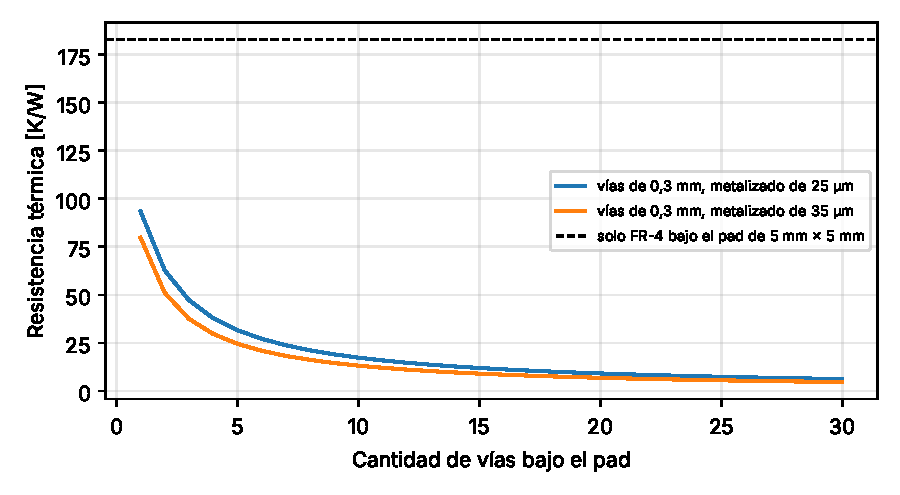
\includegraphics[width=0.85\textwidth]{resistencia_vias.pdf}
  \caption[Resistencia térmica de un conjunto de vías.]{Resistencia térmica de un conjunto de vías de \SI{0,3}{\milli\metre} en paralelo con el FR-4 bajo un pad de \SI{5}{\milli\metre}\,$\times$\,\SI{5}{\milli\metre}, en una placa de \SI{1,6}{\milli\metre} (cálculo propio).}\label{fig:termica-vias}
\end{figure}

\subsection{Camino hasta la estructura}\label{sec:termica-camino}

En una pila PC/104 no hay una placa madre: el calor llega a la estructura por los cuatro separadores de las esquinas (Capítulo~\ref{cap:pc104}). Cada separador aporta la resistencia de su cuerpo y la de las uniones atornilladas.

\subsubsection{Uniones atornilladas}

La NASA publica conductancias de uniones atornilladas que dependen del tamaño del tornillo y del par: por ejemplo, \SI{3,51}{\watt\per\kelvin} para un tornillo de 1/4--28 sobre una superficie chica y rígida y \SI{1,054}{\watt\per\kelvin} sobre superficies grandes y delgadas, y \SI{0,21}{\watt\per\kelvin} y \SI{0,105}{\watt\per\kelvin} para un tornillo 2--56 en los mismos dos casos~\cite{nasasoa}. Un ensayo de Goddard sobre una caja electrónica real en vacío mostró que los datos de catálogo, medidos en muestras chicas a presión alta, sobrestiman lo que logra una unión atornillada real, porque con tornillos solo en el perímetro el centro se separa. Los materiales de interfaz mejoraron la conductancia entre 1,2 y 28 veces según el material; el mejor (NuSil 2946) exigió unos \SI{0,5}{\milli\metre} de espesor inicial y tiene requisitos de manejo para el control de contaminación~\cite{steinfeld23}. Los rellenos térmicos comerciales que cita la NASA tienen conductividades de \SI{5}{\watt\per\metre\per\kelvin} y \SI{6}{\watt\per\metre\per\kelvin}~\cite{nasasoa}.

\subsubsection{Estimación para una pila PC/104}

Se estima la conductancia de los cuatro separadores con los datos anteriores. Hipótesis (todas propias, a confirmar con la estructura real): separadores de aluminio ($k = \SI{218}{\watt\per\metre\per\kelvin}$~\cite{guerra18}) de \SI{5}{\milli\metre} de diámetro exterior, \SI{3,2}{\milli\metre} interior y \SI{15}{\milli\metre} de largo (separación típica entre módulos, Tabla del Capítulo~\ref{cap:pc104}), con dos uniones atornilladas por separador cuya conductancia se toma como la del tornillo chico de la NASA, \SI{0,105}{\watt\per\kelvin} y \SI{0,21}{\watt\per\kelvin}. El cuerpo del separador aporta \SI{0,17}{\watt\per\kelvin}, y la Tabla~\ref{tab:termica-camino} resume el resultado.

\begin{table}[H]
  \centering
  \caption[Estimación de la conductancia de los separadores.]{Estimación (cálculo propio) del camino por cuatro separadores de aluminio, con dos uniones atornilladas cada uno.}\label{tab:termica-camino}
  \begin{tabular}{@{}*{4}{>{\centering\arraybackslash}p{3.5cm}}@{}}
    \toprule
    Conductancia por unión [W/K] & $R$ por separador [K/W] & $G$ de los cuatro [W/K] & $\Delta T$ con \SI{2}{\watt} [K] \\
    \midrule
    \num{0,105} & \num{25,0} & \num{0,160} & \num{12,5} \\
    \num{0,21}  & \num{15,5} & \num{0,259} & \num{7,7}  \\
    \bottomrule
  \end{tabular}
\end{table}

Conviene leer estos números con cuidado. Primero, las uniones dominan la resistencia: más de la mitad de $R$ está en ellas y no en el aluminio, de modo que el torque y las superficies de contacto importan más que el material del separador. Segundo, la conducción por los separadores (\num{0,16} a \SI{0,26}{\watt\per\kelvin}) es solo de 1,7 a 2,7 veces el intercambio radiante de una cara de la placa (\SI{0,095}{\watt\per\kelvin}, Sección~\ref{sec:termica-rad}), lo que confirma que no se puede ignorar la radiación interna. Tercero, esta estimación es el salto de temperatura entre la placa y la estructura, y se suma al de la placa hasta el separador y al de las vías.

\subsection{Un caso de referencia: amplificador de \SI{2}{\watt}}\label{sec:termica-guerra}

Guerra y colaboradores modelaron la electrónica de un CubeSat de \SI{10}{\centi\metre}, con tres placas, una placa de RF y cuatro varillas de aluminio como soporte, con ANSYS Icepak~\cite{guerra18}. Cada placa se modeló como diez capas de cobre en FR-4 (\SI{1,6}{\milli\metre} en total) y las varillas llevan una resistencia adicional en cada placa por la baja conductancia de contacto. La Tabla~\ref{tab:termica-guerra} resume sus resultados con un amplificador de \SI{2}{\watt}. La fuente toma \SI{80}{\celsius} como límite recomendado para ese componente~\cite{guerra18}.

\begin{table}[H]
  \centering
  \caption[Temperaturas de un amplificador de 2 W en un CubeSat.]{Resultados de Guerra y colaboradores para un amplificador que disipa \SI{2}{\watt} en un CubeSat de \SI{10}{\centi\metre}~\cite{guerra18}. El primer valor corresponde a una operación de \SI{10}{\second} cada \SI{20}{\second}, y el segundo, a \SI{5}{\second} cada \SI{20}{\second}.}\label{tab:termica-guerra}
  \begin{tabular}{@{}lc@{}}
    \toprule
    Configuración & Temperatura máxima del amplificador [$^\circ$C] \\
    \midrule
    Sin tira térmica         & 131 y 124 \\
    Con tira de grafito      & 103 y 99 \\
    \bottomrule
  \end{tabular}
\end{table}

La tira térmica es una lámina de grafito pirolítico de \SI{25}{\micro\metre} plegada en bucle, y baja unos \SI{25}{\celsius} la temperatura, pero el amplificador sigue por encima del límite de \SI{80}{\celsius}~\cite{guerra18}. Con el amplificador apagado, el componente más caliente era el procesador, a unos \SI{63}{\celsius}~\cite{guerra18}. La lección es que la etapa de potencia de RF es un punto caliente concentrado, y que un camino térmico pensado para el promedio de la placa no alcanza. Es un caso de otro satélite, con otra geometría, y no se puede trasladar directamente.

\subsection{Reglas de diseño térmico}\label{sec:termica-reglas}

La Tabla~\ref{tab:termica-reglas} resume las reglas propuestas para la placa del PI\@. Como en el capítulo anterior, se indica el origen de cada una.

\begin{table}[H]
  \centering
  \caption[Reglas de diseño térmico propuestas.]{Reglas de diseño térmico propuestas para la placa del PI y origen de cada una.}\label{tab:termica-reglas}
  \begin{tabular}{@{}>{\raggedright\arraybackslash}p{3.1cm}>{\raggedright\arraybackslash}p{7.2cm}>{\raggedright\arraybackslash}p{4.3cm}@{}}
    \toprule
    Tema & Regla & Origen \\
    \midrule
    Pad térmico & Soldar el pad del componente con al menos \SI{50}{\percent} de cobertura, y conectarlo a los planos con unión continua, sin alivio térmico. & Fuente~\cite{tislma002} \\
    Vías térmicas & Entre cinco y nueve vías bajo el pad como mínimo, de \SI{0,33}{\milli\metre} o menos, con máscara del lado del componente; más vías si la potencia lo exige. & Fuente~\cite{tislma002}; cálculo propio (Figura~\ref{fig:termica-vias}) \\
    Cobre & Planos de cobre internos continuos y de mayor espesor para repartir el calor hacia las esquinas. & Fuentes~\cite{nasasoa}; cálculo propio (Tabla~\ref{tab:termica-keq}) \\
    Camino a la estructura & Llevar el calor del componente hacia los agujeros de montaje; apretar las uniones con el torque especificado. & Cálculo propio (Tabla~\ref{tab:termica-camino}) y~\cite{steinfeld23} \\
    Punto caliente & Si la potencia es de varios vatios, prever una tira térmica o un relleno de interfaz hasta la estructura. & Fuentes~\cite{guerra18,nasasoa} \\
    Materiales de interfaz & Elegirlos con el criterio de desgasificación de la CDS\@. & Capítulo~\ref{cap:cds}; práctica \\
    Radiación & No contar con la radiación interna como sumidero: el calor debe salir por la estructura. & Cálculo propio (Sección~\ref{sec:termica-rad}) \\
    \bottomrule
  \end{tabular}
\end{table}

\verificar{si el equipo de la estructura del satélite admite una tira térmica o un relleno de interfaz entre la placa y los rieles, y qué materiales cumplen la desgasificación de la CDS}

%--------------------------------------------------------------------
\section{Blindaje y compatibilidad electromagnética}\label{sec:emi}

\subsection{Qué se necesita y qué normas existen}\label{sec:emi-normas}

En el relevamiento de la CDS del Capítulo~\ref{cap:cds} la RF aparece desde la seguridad (inhibiciones y licencias), y no se relevó un requisito numérico de emisión o inmunidad electromagnética. Para satélites en general, la norma ECSS-E-ST-20\nobreakdash-07C Rev.~2 (3 de enero de 2022), \emph{Electromagnetic compatibility}, fija requisitos detallados de sistema, condiciones de ensayo, verificación a nivel de sistema y métodos de ensayo de subsistemas y equipos, con límites informativos en un anexo~\cite{ecss2007}. Se consultó solo su página descriptiva. \verificar{los requisitos de EMC y de emisiones espurias que impondrán el proveedor de lanzamiento y la licencia de frecuencias, y si se tomará alguna norma como guía}

Para la cadena del PI hay tres necesidades concretas. La primera es que la etapa de potencia no se realimente y oscile (Sección~\ref{sec:emi-aislacion}). La segunda es que el transmisor no interfiera al receptor ni a la electrónica digital del satélite, cuya fuente de ruido son además los reguladores conmutados y los relojes. La tercera es que los armónicos y las espurias que genera el amplificador no salgan a la antena, tarea del segundo filtro de la cadena. Las dos primeras son de layout y blindaje, y son el tema de esta sección.

\subsection{Fundamentos del blindaje}\label{sec:emi-fundamentos}

La efectividad de blindaje (SE, \emph{shielding effectiveness}) es la relación en decibeles entre la señal con y sin blindaje, y se descompone en pérdida por absorción $A$ y por reflexión $R$~\cite{rosehulman}:
\begin{equation}\label{eq:emi-se}
  \mathrm{SE} = A + R, \qquad A = 8{,}69\,\frac{t}{\delta}, \qquad \delta = \sqrt{\frac{2}{\omega\mu\sigma}}, \qquad R = 20\log \frac{Z_w}{4 Z_m},
\end{equation}
con $t$ el espesor del blindaje, $\delta$ la profundidad de penetración, $Z_w \approx \SI{377}{\ohm}$ la impedancia de onda (caso de onda plana) y $Z_m = \sqrt{\omega\mu/\sigma}$ la del metal~\cite{rosehulman}. Las fuentes consultadas dan la reflexión de campo cercano (eléctrico y magnético) con constantes que no se pudieron leer, por lo que aquí solo se usa el caso de onda plana.

\begin{table}[H]
  \centering
  \caption[Blindaje de una lámina de 0,2 mm de cobre o aluminio.]{Profundidad de penetración y pérdidas de una lámina de \SI{0,2}{\milli\metre} (cálculo propio con la ecuación~\eqref{eq:emi-se}, onda plana). Conductividades: cobre \SI{5,8e7}{\siemens\per\metre} y aluminio \SI{3,7e7}{\siemens\per\metre}~\cite{rosehulman}.}\label{tab:emi-lamina}
  \begin{tabular}{@{}llcccc@{}}
    \toprule
    Material & $f$ [MHz] & $\delta$ [\si{\micro\metre}] & $Z_m$ [m$\Omega$] & $A$ [dB] & $R$ [dB] \\
    \midrule
    Cobre    & 145 & \num{5,49} & \num{4,44} & 317 & \num{86,5} \\
    Cobre    & 435 & \num{3,17} & \num{7,70} & 548 & \num{81,8} \\
    Aluminio & 145 & \num{6,87} & \num{5,56} & 253 & \num{84,6} \\
    Aluminio & 435 & \num{3,97} & \num{9,63} & 438 & \num{79,8} \\
    \bottomrule
  \end{tabular}
\end{table}

La conclusión de la Tabla~\ref{tab:emi-lamina} es que en VHF/UHF cualquier lámina metálica de décimas de milímetro es, en la práctica, un blindaje perfecto: la absorción es de cientos de decibeles y la reflexión supera los \SI{80}{\decibel}. Lo que limita la efectividad real son las aberturas y las costuras.

\subsection{Aberturas y costuras}\label{sec:emi-aberturas}

Una abertura de dimensión mayor $l$ deja pasar la señal de forma apreciable por encima de una frecuencia de corte $f_c = \SI{15000}{\mega\hertz} / l$, con $l$ en centímetros. Por debajo, la reflexión es aproximadamente $R \approx 20\log (f_c/f)$, y la absorción a través del agujero para un espesor $t$ es de $27{,}3\,t/l$ dB en una abertura rectangular~\cite{rosehulman}. Con varias aberturas iguales la efectividad cae $10\log N$ dB~\cite{rosehulman}. Como $f_c = c/2l$, la expresión de reflexión equivale a $20\log\,(\lambda/2l)$ (derivación propia). La Tabla~\ref{tab:emi-aberturas} y la Figura~\ref{fig:emi-aberturas} muestran el resultado.

\begin{table}[H]
  \centering
  \caption[Efectividad de blindaje limitada por una abertura.]{Efectividad de blindaje limitada por una abertura de dimensión mayor $l$ (cálculo propio, $R \approx 20\log (f_c/f)$ con $f_c = \SI{15000}{\mega\hertz}/l$).}\label{tab:emi-aberturas}
  \begin{tabular}{@{}rcccc@{}}
    \toprule
    $l$ [mm] & $f_c$ [GHz] & SE a \SI{145}{\mega\hertz} [dB] & SE a \SI{435}{\mega\hertz} [dB] & SE a \SI{870}{\mega\hertz} [dB] \\
    \midrule
    1  & 150  & \num{60,3} & \num{50,8} & \num{44,7} \\
    5  & 30   & \num{46,3} & \num{36,8} & \num{30,8} \\
    10 & 15   & \num{40,3} & \num{30,8} & \num{24,7} \\
    20 & 7,5  & \num{34,3} & \num{24,7} & \num{18,7} \\
    \bottomrule
  \end{tabular}
\end{table}

\begin{figure}[H]
  \centering
  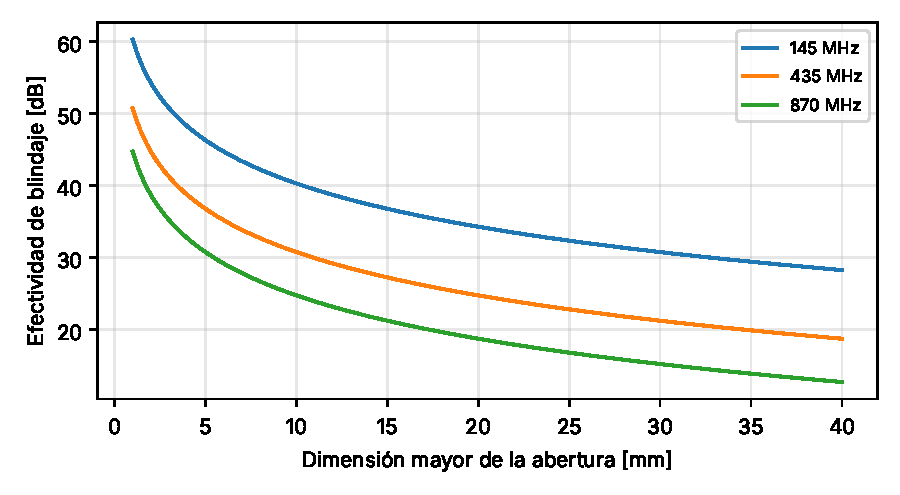
\includegraphics[width=0.85\textwidth]{se_apertura.pdf}
  \caption[Efectividad de blindaje frente al tamaño de la abertura.]{Efectividad de blindaje limitada por una abertura, según su dimensión mayor, a tres frecuencias (cálculo propio con el modelo de la Sección~\ref{sec:emi-aberturas}).}\label{fig:emi-aberturas}
\end{figure}

El modelo es una cota simple: trata la abertura como un orificio aislado en una pared plana y no incluye el espesor ni el acople con los componentes internos. Con una tapa de \SI{20}{\milli\metre} de costura abierta se obtiene a \SI{435}{\mega\hertz} unos \SI{25}{\decibel}, que es poco. Una costura fina, en cambio, se trata mejor como una hilera de aberturas de longitud igual a la separación entre contactos.

\subsection{Blindaje a nivel de placa}\label{sec:emi-placa}

El blindaje de una etapa de RF sobre la placa se realiza con una carcasa metálica soldada a un marco de cobre, unido al plano de masa inferior con una hilera de vías. El artículo de síntesis del anteproyecto de guía IEEE P2716 sobre blindajes de placa confirma que las aberturas (rendijas entre la tapa y el marco, huecos en las esquinas, orificios de ventilación) son un factor mayor en la efectividad real, y que las vías demasiado separadas pueden producir fugas, aunque no da una regla de separación~\cite{dawson23}. Una fuente divulgativa propone un paso de vías menor que $\lambda/20$, con carcasas de acero estañado o alpaca de \num{0,2} a \SI{0,3}{\milli\metre}, y da \num{40} a \SI{60}{\decibel} de efectividad para una carcasa y \num{40} a \SI{70}{\decibel} de aislación entre dos adyacentes~\cite{rfessentialsbls}. Esa fuente no cita referencias, y se la toma con cautela.

Aplicando el modelo de la Sección~\ref{sec:emi-aberturas} al espacio entre vías, un paso de $\lambda/20$ corresponde a una abertura de $l = \lambda/20$ y a una efectividad de $20\log 10 = \SI{20}{\decibel}$ exactamente, sin importar la frecuencia (cálculo propio). Es decir, $\lambda/20$ es un mínimo, y para llegar a \SI{40}{\decibel} hace falta un paso diez veces menor ($\lambda/200$). La Tabla~\ref{tab:emi-paso} muestra los números para \SI{435}{\mega\hertz} y para su segundo armónico.

\begin{table}[H]
  \centering
  \caption[Efectividad del vallado de vías según su paso.]{Efectividad estimada del vallado de vías de masa según el paso (cálculo propio, $20\log (\lambda/2p)$).}\label{tab:emi-paso}
  \begin{tabular}{@{}rcc@{}}
    \toprule
    Paso $p$ [mm] & SE a \SI{435}{\mega\hertz} [dB] & SE a \SI{870}{\mega\hertz} [dB] \\
    \midrule
    34  & \num{20,1} & \num{14,1} \\
    17  & \num{26,1} & \num{20,1} \\
    10  & \num{30,7} & \num{24,7} \\
    5   & \num{36,8} & \num{30,7} \\
    2   & \num{44,7} & \num{38,7} \\
    \bottomrule
  \end{tabular}
\end{table}

\begin{description}
  \item[Material de la carcasa.] Una carcasa de acero estañado trae el problema de los filamentos de estaño de la Sección~\ref{sec:layout-espacio}: la NASA recomienda evitar los acabados de estaño puro~\cite{brusse}. La alpaca (\emph{nickel silver}) figura como alternativa en la fuente anterior~\cite{rfessentialsbls}. \verificar{el acabado de las carcasas disponibles}
  \item[Líneas de continua y control.] La fuente divulgativa recomienda filtrar las líneas de alimentación y control en la pared del blindaje con capacitores pasantes o pines filtrados~\cite{rfessentialsbls}, para que el cable no sea la abertura.
  \item[Calor.] Una carcasa cerrada sobre el amplificador cubre justo el punto caliente; la tapa no debe ser el único camino de calor (Sección~\ref{sec:termica-camino}).
  \item[Desgasificación.] Las juntas conductoras, los absorbentes y los adhesivos del blindaje deben cumplir el criterio de TML y CVCM de la CDS (Sección~\ref{sec:layout-outgassing}). \verificar{TML y CVCM de los materiales de blindaje que se elijan}
\end{description}

\subsection{Aislación entre etapas de la cadena}\label{sec:emi-aislacion}

Un amplificador con ganancia $G$ y una trayectoria parásita de aislación $I$ entre su salida y su entrada forman un lazo de realimentación con ganancia $G - I$ (ambas en decibeles). Para que el lazo no oscile hace falta $I > G$ con un margen. Por ejemplo, con $G = \SI{20}{\decibel}$ y un margen de \SI{10}{\decibel}, la aislación necesaria es de \SI{30}{\decibel}. Es un criterio propio que no sustituye un análisis de estabilidad como el que se hace con los parámetros S del dispositivo~\cite{gonzalez}. \verificar{la ganancia de la etapa del PI y el margen de estabilidad que se exigirá}

La misma fuente divulgativa estima una aislación natural de \num{30} a \SI{50}{\decibel} para etapas separadas por más de \SI{20}{\milli\metre} y de \num{40} a \SI{70}{\decibel} con carcasas adyacentes~\cite{rfessentialsbls}. Si esos órdenes de magnitud fueran correctos, una cadena filtro--amplificador--filtro en línea recta cumpliría el ejemplo de \SI{30}{\decibel} sin blindaje, y la carcasa sería necesaria si la ganancia es mayor o si el espacio obliga a juntar etapas. Esto debe confirmarse con la ganancia real y por simulación o medición.

\subsection{Reglas de blindaje y EMC}\label{sec:emi-reglas}

\begin{table}[H]
  \centering
  \caption[Reglas de blindaje y EMC propuestas.]{Reglas de blindaje y EMC propuestas para la placa del PI y origen de cada una.}\label{tab:emi-reglas}
  \begin{tabular}{@{}>{\raggedright\arraybackslash}p{3.1cm}>{\raggedright\arraybackslash}p{7.2cm}>{\raggedright\arraybackslash}p{4.3cm}@{}}
    \toprule
    Tema & Regla & Origen \\
    \midrule
    Material & Cualquier lámina metálica de décimas de milímetro basta: las pérdidas del material no limitan. & Cálculo propio (Tabla~\ref{tab:emi-lamina}) \\
    Aberturas & Mantener las aberturas y las costuras lo más cortas posible; tratar cada costura como una hilera de aberturas. & Fuente~\cite{rosehulman}; cálculo propio \\
    Vallado de vías & Paso de vías menor que $\lambda/20$ como mínimo (\SI{20}{\decibel}), y del orden de $\lambda/100$ o menos si se busca \SI{35}{\decibel} o más. & Cálculo propio y~\cite{rfessentialsbls} \\
    Carcasa & Alpaca u otro acabado sin estaño puro, soldada al marco de cobre. & Fuentes~\cite{brusse,rfessentialsbls} \\
    Líneas de continua & Filtrar las líneas que atraviesan el blindaje. & Fuente~\cite{rfessentialsbls} \\
    Aislación & Cumplir $I > G +$ margen, con $I$ medida o simulada. & Cálculo propio \\
    Materiales & Elegir juntas y absorbentes que cumplan TML y CVCM de la CDS\@. & Capítulo~\ref{cap:cds} \\
    \bottomrule
  \end{tabular}
\end{table}

%--------------------------------------------------------------------
\section{Síntesis para el Proyecto Integrador}\label{sec:termica-sintesis}

\begin{itemize}
  \item En vacío, el calor de la etapa de potencia solo sale por conducción hasta la estructura, y la conducción de la placa es buena en el plano y mala en espesor: hacen falta vías térmicas, entre cinco y nueve como mínimo.
  \item Los separadores y sus uniones atornilladas fijan el salto de temperatura entre la placa y la estructura; con las hipótesis de este capítulo es de unos \num{8} a \SI{12}{\kelvin} para \SI{2}{\watt}.
  \item Un amplificador de \SI{2}{\watt} llegó a \SI{131}{\celsius} sin tira térmica en un caso publicado, por lo que la potencia que disipe el PI y su límite de temperatura son datos de entrada críticos.
  \item En VHF/UHF el material del blindaje no es el problema; lo son las aberturas, las costuras y el paso de las vías. Un paso de $\lambda/20$ da solo \SI{20}{\decibel}.
  \item Los materiales de interfaz, las juntas y los acabados deben cumplir la desgasificación de la CDS y evitar el estaño puro.
\end{itemize}
